%LET'S GO TEAM!!! ONE LESS SECTION
%We are unstoppppable --> DAB DAB DAB

To design Astrea constellation the orbit parameters must be decided following the established requirements. As seen in the previous sections, there are different types of constellation that must be considered when selecting those parameters. The main requirement in the bases of this chapter is to fulfil global coverage of the Earth. Therefore all the possible solutions have to be tested to ensure they pass this specification.

\subsubsubsection*{Method Bases and Results}
The method consist in evaluating all the possible combinations between the variables listed in the table~\ref{t:CovVar} within established margins and testing them to know if they fulfil the determined conditions that ensure global coverage. The conditions considered to asses this global coverage and the details of the method can be reviewed in \cite[Chapter 3, Section 5]{annex1}. %Figure~\ref{fig:AngleSSatFoot} shows the complete algorithm for this method.

\begin{table}[H]
\centering
\begin{tabular}{|c|l|c|l|}
\hline
$$typeC$$     & Type of constellation    & $$in$$  & Inclination angle {[}º{]} \\ \hline
$\varepsilon$ & Elevation angle {[}º{]}  & $n_{p}$ & Number of Planes                          \\ \hline
$$h$$         & Height  {[}km{]}  & $N_{pp}$ & Number of Satellites per plane            \\ \hline
\end{tabular}
\caption{Coverage Testing Method main Variables}
\label{t:CovVar}
\end{table}  

A MATLAB routine has been developed (see details in the same attachment) to see the evolution of a satellite network configuration regarding the variation of the orbital parameters. With this code, the optimum configuration can be obtained given the chosen requirements. The configurations that will be later considered to perform an analysis of weighted parameters are extracted from this routine.

To visually check the coverage obtained, the ground track of three configurations have been plotted. The figure~\ref{fig:gt210} shows one of them, the others can be found in the \cite[Chapter 3, Section 5]{annex1}. 

\begin{figure}[H] %[b] % h / H / b / t
	\centering
	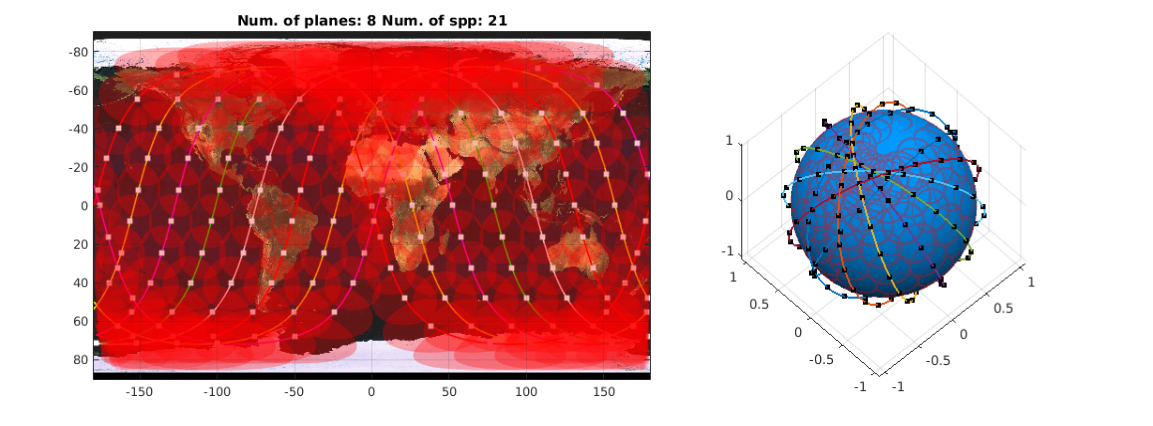
\includegraphics[width=.8\textwidth]{./testing/WB210.png}\\
	\caption[Ground track and spherical representation of a 210º Walker Delta]{Ground track and spherical representation of a 210º Walker Delta configuration}
	\label{fig:gt210}
\end{figure}